\section{Introduction}
% what is ``Space subdivision''
Subdivision is the process of partitioning a space $\mathcal{S}$, according to a provided set of level-curves $\mathcal{C}$ in that space, into a set of faces $\mathcal{F}$.
%% \footnote{for simplicity, level-curves will be refered to as curves in the rest of the document.} 

\[ \mathit{subdivision}(\mathcal{C}): \mathcal{S} \xrightarrow[]{decompose} \mathcal{F}\left(\mathcal{C}\right) \]

Figure~\ref{fig:intro_curvesPartitioning1} shows an example of a planar subdivision (where $\mathcal{S}$ is two dimensional), according to a set of curves containing six straight lines.
% what is it useful for? some application?
The process of subdivision provides an abstraction of the space.
Such an abstraction potentially facilitates some geometric processes required on that space.

\begin{figure}%[!ht]
  \centering
  \begin{subfigure}{.4\textwidth}
    
\includegraphics[width=\textwidth]{figures/intro_curves1.png}
    \caption{curves} \label{subfig:intro_curves1}
  \end{subfigure}%
  \quad \quad \quad%
  \begin{subfigure}{.4\textwidth}
    
\includegraphics[width=\textwidth]{figures/intro_partitioning1.png}
    \caption{partitionaing} \label{subfig:intro_partitioning1}
  \end{subfigure}%
  \caption[xxx]
          {A planar subdivision, over a set of six straight lines.
          Figure~\ref{subfig:intro_curves1} shows the set of curves, and the ``faces'' resulting from partitioning are color coded in figure~\ref{subfig:intro_partitioning1}.}
  \label{fig:intro_curvesPartitioning1}
\end{figure}

%%%%%%%%%%%%%%%%%%%%%%%%%%%%%%%%%%%%%%%%%%%%%%%%%%%%%%%%%%%%%%%%%%%%%%%%%%%%%%%%
\subsection{Problem Statement}

Here we define some of the terminologies, and briefly explain some of the challenges and requirements.

\paragraph{Curves}
A curve set $\mathcal{C}$ contains the level-curves of some multivariable functions $f(X)$ defined over a space $\mathcal{S}$.
\[
\mathcal{C} = \lbrace c_i \mid c_i: f_i(X)=0, i \in I, \text{$I$: index set of $\mathcal{C}$} \rbrace
\]

\paragraph{Faces}
A face is the ``interior'' region of a ``Jodan Curve''.
The Jordan curve in our problem setting could be a compilation of curves.
%WIKI: a plane simple closed curve is a non-self-intersecting continuous loop in the plane (aka Jordan curve).
%WIKI: The Jordan curve theorem asserts that every Jordan curve divides the plane into an "interior" region bounded by the curve and an "exterior" region containing all of the nearby and far away exterior points,
The set of faces $\mathcal{F}$ satisfies following conditions:
\[
\begin{array}{l}
  \nexists face_i , face_j \in \mathcal{F}, \quad face_i \cap face_j \neq \emptyset \quad \text{($\cap$: geometric intersection)}\\
  \quad \\
  \displaystyle\bigcup_{ i \in \mathcal{I} } face_i \subset \mathcal{S} \quad \text{($I$: index set of $\mathcal{F}$, and $\cup$: geometric union)}
\end{array}
\]

\paragraph{Membership and neighborhood of faces}
Two important method that the face data structure must support are the \emph{membership} and \emph{neighborhood} functions.
Membership is a function of points which returns the face that encompass a given point.
That is to say, membership function identifies the ``interior'' region of the faces.
Neighborhood is a function of faces and returns all other faces that are neighboring the input face by the mean of [at least] one shared edge in their boundaries.
%% While membership function depends on geometric processes, neighborhood function is often handled by the attributes of the date structures.

\[
\begin{array}{l}
  \mathit{member}\left(point\right) = face_i \quad, face_i \text{ encompasses the } point \\
  \mathit{neighbor}\left(face_i\right) = \lbrace  face_j \mid \exists edge_k, edge_k \in face_i \land edge_k \in face_j \rbrace\\
\end{array}
\]

\paragraph{Unbounded faces}
The fact that $\bigcup face_i$ is a proper subset of and not equal to $\mathcal{S}$, raise a question about the exterior region which does not belong to any of the normal faces.
The exterior region could be treated either as separate unbounded faces (as in figure~\ref{subfig:intro_unboundedFaces_b}), or a unified single unbounded face (as in figure~\ref{subfig:intro_unboundedFaces_c}).
Following the latter approach, we treat the union of all the exterior region as a single unbounded face.

\begin{figure}%[!ht]
  \centering
  \begin{subfigure}{.32\textwidth}
    
\includegraphics[width=\textwidth]{figures/intro_curves1.png}
    \caption{curves} \label{subfig:intro_unboundedFaces_a}
  \end{subfigure}%
  ~%
  \begin{subfigure}{.32\textwidth}
    
\includegraphics[width=\textwidth]{figures/intro_unboundedFaces_b.png}
    \caption{separate faces} \label{subfig:intro_unboundedFaces_b}
  \end{subfigure}%
  ~%
  \begin{subfigure}{.32\textwidth}
    
\includegraphics[width=\textwidth]{figures/intro_unboundedFaces_c.png}
    \caption{unified face} \label{subfig:intro_unboundedFaces_c}
  \end{subfigure}%
  \caption[xxx]
          {Two approaches for dealing with the unbounded exterior region.
          In this work we take the approach in figure~\ref{subfig:intro_unboundedFaces_c}, that is to say, treating the whole exterior region as one unbounded face.}
  \label{fig:intro_unboundedFaces}
\end{figure}

%%%%%%%%%%%%%%%%%%%%%%%%%%%%%%%%%%%%%%%%%%%%%%%%%%%%%%%%%%%%%%%%%%%%%%%%%%%%%%%%
\subsection{Background}
\td{I still can't believe this problem has not been solved! :(}
%% Where the space $\mathcal{S}$ is two dimensional and the curve set $\mathcal{C}$ contains the level curves of only linear functions ($f(X)$).
%% \[ \mathcal{C} = \lbrace c_i \mid c_i: ax_1+bx_2+c=0, i \in I, \text{$I$: index set of $\mathcal{C}$} \rbrace \]
%% Consequently every face is a polygon bounded to line segments.


%%%%%%%%%%%%%%%%%%%%%%%%%%%%%%%%%%%%%%%%%%%%%%%%%%%%%%%%%%%%%%%%%%%%%%%%%%%%%%%%
\subsection{This work}

This work aims at studying the subdivision problem in the presence of circles.
After identifying the limitation of the existing solutions in handling the more generic cases, challanges are identified and addressed.
Figure~\ref{fig:intro_curvesPartitioning2} illustrates an example of a planar subdivision in the presence of circles.
This work relies on the following assumptions:
\begin{description}
\item [Dimension] the space is a two dimensional plane.
\item [Curves] the set $\mathcal{C}$ contains levels curves resulted from either linear functions (straight lines as an example of an unbounded class) or conic sections (circles as an example of a bounded class).
\item [Redundancy] if two curves were identical, their intersection would be the same curve which is beyond a finite set of points.
  In order to prevents the intersection procedure yielding a result other than a finite set of points, redundant curves are rejected so that;
  \[ \nexists c_i , c_j \in \mathcal{C}, \quad c_i = c_j \]
\end{description}

\begin{figure}%[!ht]
  \centering
  \begin{subfigure}{.4\textwidth}
    
\includegraphics[width=\textwidth]{figures/intro_curves2.png}
    \caption{curves} \label{subfig:intro_curves2}
  \end{subfigure}%
  \quad \quad \quad%
  \begin{subfigure}{.4\textwidth}
    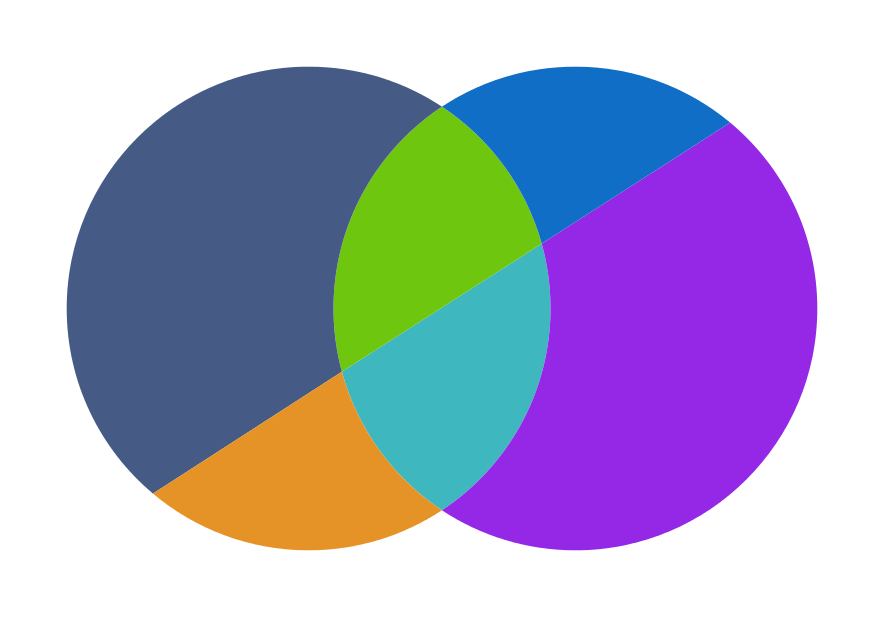
\includegraphics[width=\textwidth]{figures/intro_partitioning2.png}
    \caption{partitionaing} \label{subfig:intro_partitioning2}
  \end{subfigure}%
  \caption[xxx]
          {A planar subdivision, over a set of curves containing a straight line and two circles.
          Figure~\ref{subfig:intro_curves2} shows the set of curves, and the ``faces'' resulting from partitioning are color coded in figure~\ref{subfig:intro_partitioning2}.}
  \label{fig:intro_curvesPartitioning2}
\end{figure}

%%%%%%%%%%%%%%%%%%%%%%%%%%%%%%%%%%%%%%%%
\subsubsection{Challenges}

Introducing circles raises challenges from the meta-algorithm of subdivision, all the way to sub-procedures within.
Most of these challenges, as we'll see, are based on three essential differences between lines and circles;
\begin{inparaenum}[\itshape i\upshape)]
  \item \emph{boundness}: a circle could be enclosed within a closed curve (i.e. a Jordan Curve), while a line stretches to infinity;
  \item \emph{closed curve}: unlike a line, a circle itself is a closed curve and alone could result in bounded faces; and 
  \item \emph{segment representation}: while a segment of a line could be represented by a vector, a segment of a circle is represented by an arc.
\end{inparaenum}


\paragraph{None intersecting circles}
If a line does not intersect with any other curves in the curve set $\mathcal{C}$, it could be safely discarded as it would not result in any bounded region.
On the other hand, a circle which does not have any intersection point with other curves would result in a bounded region that should be counted and identified as a face.
That is to say, in the absence of circles it is safely assumed that the intersection points are well representing all the edges, and consequently all the faces.
We tackle this problem by introducing dummy intersection points over non-intersecting circles.

\paragraph{Sorting nodes over curves}
In order to identify the edges resulting from a curve, it is essential to be able to geometrically sort the intersection points over the curve.
For lines it suffices to sort the points according to their $x$ (or $y$) values.
This does not hold for circles.
To this end, we employ a univariate represetation for curves (presented in appendix~\ref{app:alternativeRep}).

\paragraph{Edges are no longer vectors}
A key information in face identification is the ability to follow a geometric path of edges that bound a face.
This is an iterative process of finding the correct successor to an edge, until the sequence of edges form a closed curve, which represents the face.
The correct successor is identified by its departing angle with respect to the arriving angle of the last edge.
In the case of only lines, the arriving and departing angles of edges are equivalent to the slope of the line.
But in the case of arc shaped edges, we have to employ the derivatives of the curve and the intersection point to find the correct successor.

\paragraph{Holes}
A new feature that appears in the presence of circles is the holes.
That is to say, a face could have a non-continuous sequence of edges that define its boundary.
This is due to the face that a circle could be enclosed in the closed curve of a face, and creating a ``hole'' in it.
On the subdivision level, it causes the subdivision to become topologically disconnect (i.e. have separate connected components).
We approach this problem by partitioning the space according to each connected components of the subdivsion separately, and merging their results at the end.

\paragraph{Membership function}
Membership function for the subdivision of lines could be implemented through a set of tests relying on cross products, as described in \cite{de2000computational}.
The tests are to check whether if a point is located on the same side of all the bounding edges of a face.
This would only work if the edges could be represented by vectors, and if the face is convex.
As can be seen in figure~\ref{fig:intro_crossProdFail}, edges turn to arcs in the presence of circles, and potentially a face could be concave.
As an alternative we suggest the use of ``point-in-polygon'' method, which is based upon the Jordan Curve theorem.

\begin{figure} %[!ht]
    \centering
    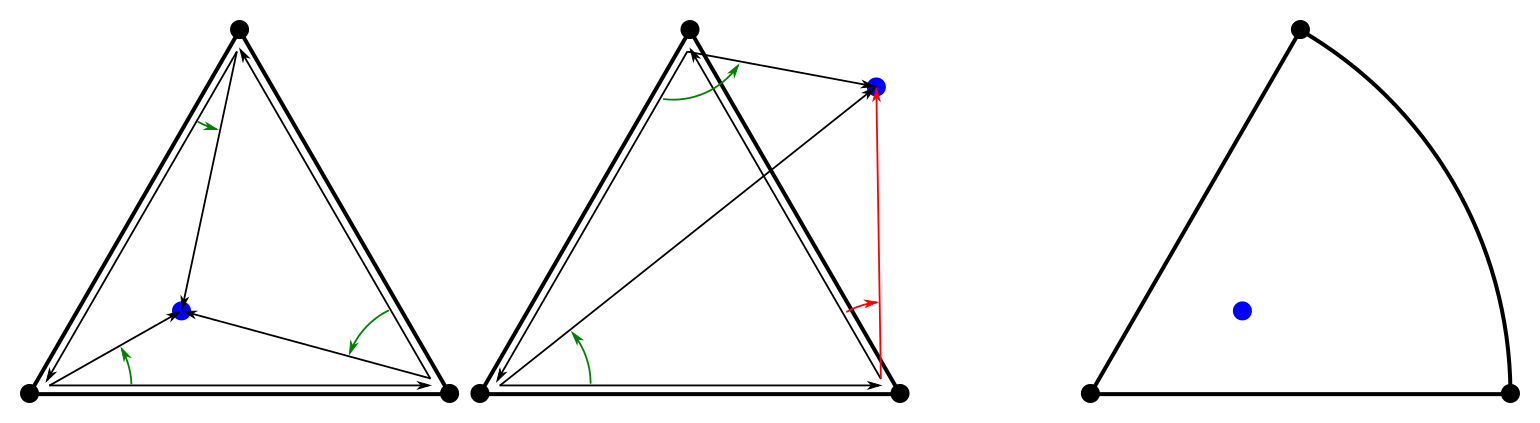
\includegraphics[width=1.\textwidth]{figures/intro_crossProdFail.png}
    \caption{Membership function for the case of only straight lines could be based on tests relying on a cross product.
    However, as the edges are no longer vectors in the presence of circles, the conventional membership procedure requires revision.}
    \label{fig:intro_crossProdFail}
\end{figure}
